\documentclass{beamer}

\mode<presentation>
{
  \usetheme{Berlin}
  \usecolortheme{orchid}
  \setbeamercovered{transparent}
}

\usepackage[english]{babel}
\usepackage[latin1]{inputenc}
\usepackage{times}
\usepackage{fontenc} 
% Or whatever. Note that the encoding and the font should match. If T1
% does not look nice, try deleting the line with the fontenc.
\usepackage{amsmath}


\beamertemplatenavigationsymbolsempty

\newcommand{\linespace}{\vskip 0.25cm}

\definecolor{MyForestGreen}{rgb}{0,0.7,0} 
\newcommand{\tableemph}[1]{{#1}}
\newcommand{\tablewin}[1]{\tableemph{#1}}
\newcommand{\tablemid}[1]{\tableemph{#1}}
\newcommand{\tablelose}[1]{\tableemph{#1}}

\definecolor{MyLightGray}{rgb}{0.6,0.6,0.6}
\newcommand{\tabletie}[1]{\color{MyLightGray} {#1}}

% The text in square brackets is the short version of your title and will be used in the
% header/footer depending on your theme.
\title{Applying Genetic Programming to\\ Bytecode and Assembly}

% Sub-titles are optional - uncomment and edit the next line if you want one.
% \subtitle{Why does sub-tree crossover work?} 

% The text in square brackets is the short version of your name(s) and will be used in the
% header/footer depending on your theme.
\author{Eric Collom}

% The text in square brackets is the short version of your institution and will be used in the
% header/footer depending on your theme.
\institute[University of Minnesota, Morris]
{
  Division of Science and Mathematics \\
  University of Minnesota, Morris \\
  Morris, Minnesota, USA
}

% The text in square brackets is the short version of the date if you need that.
\date{29 April '14,\\ UMM Senior Seminar}

% Delete this, if you do not want the table of contents to pop up at
% the beginning of each subsection:
\AtBeginSection[]
{
  \begin{frame}<beamer>
    \frametitle{Outline}
    \tableofcontents[currentsection, hideothersubsections]
  \end{frame}
}

\begin{document}

\begin{frame}
  \titlepage
\end{frame}

% For a 20-25 minute senior seminar talk you probably want something like:
% - Two or three major sections (other than the summary).
% - At *most* three subsections per section.resentation, people show regularly a "outline" frame containing the table of contents where some sections are grey (have been presented) and others are highlighted (will be presented right now).
% - Talk about 30s to 2min per frame. So there should probably be between
%   15 and 30 frames, all told.

\section*{Overview}


\subsection*{Outline}

\begin{frame}
  \frametitle{Outline}
  \tableofcontents[hideallsubsections]
\end{frame}

\section[Background]{Evolutionary Computation}

\subsection[Evolutionary Computation]{What is it?}

\begin{frame}
  \frametitle{What is Evolutionary Computation?}
  \begin{columns}
  \begin{column}{0.6\textwidth}
  \begin{itemize}
  	\item Evolutionary Computation (EC) is a a technique that is used to automate computer problem solving.
  	\item Loosely emulates evolutionary biology.
  \end{itemize}
  \end{column}
  \begin{column}{0.4\textwidth}
   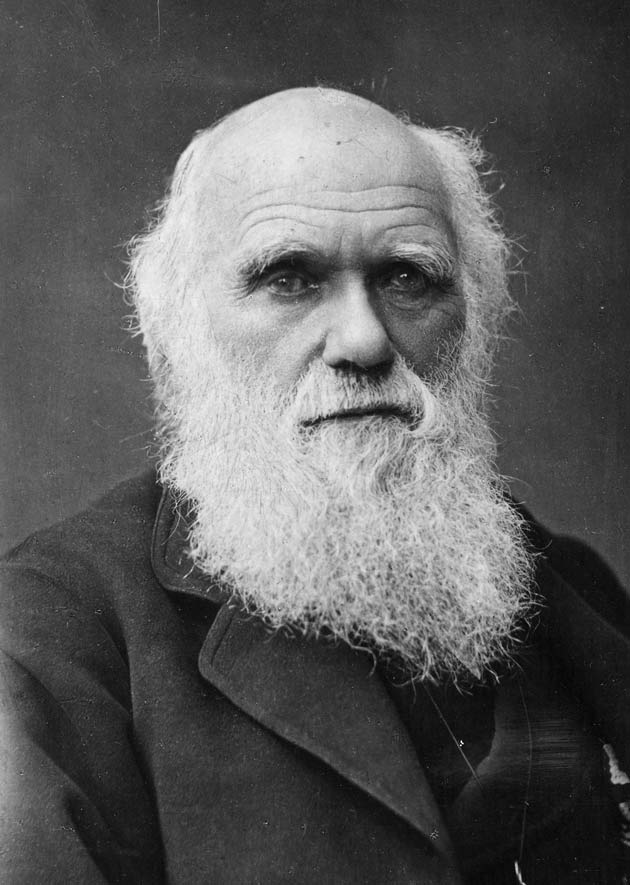
\includegraphics[width=0.95\textwidth]{Illustrations/darwin.jpg}
       \\
    \only{\tiny{Charles Darwin \\ \url{http://tinyurl.com/lqwj3wt} }}
  \end{column}
  \end{columns}
\end{frame}
\subsection[Evolutionary Computation]{How does it work?}

\begin{frame}
	\frametitle{How does it work?}
\begin{columns}[T]
\begin{column}{0.6\textwidth}
\begin{itemize}
	\item Continuous optimization \\
	\item Selection is driven by the \textit{fitness} of individuals
	\item Genetic operators mimic sexual reproduction and mutation
	
\end{itemize}
\end{column}
\begin{column}{0.4\textwidth}
   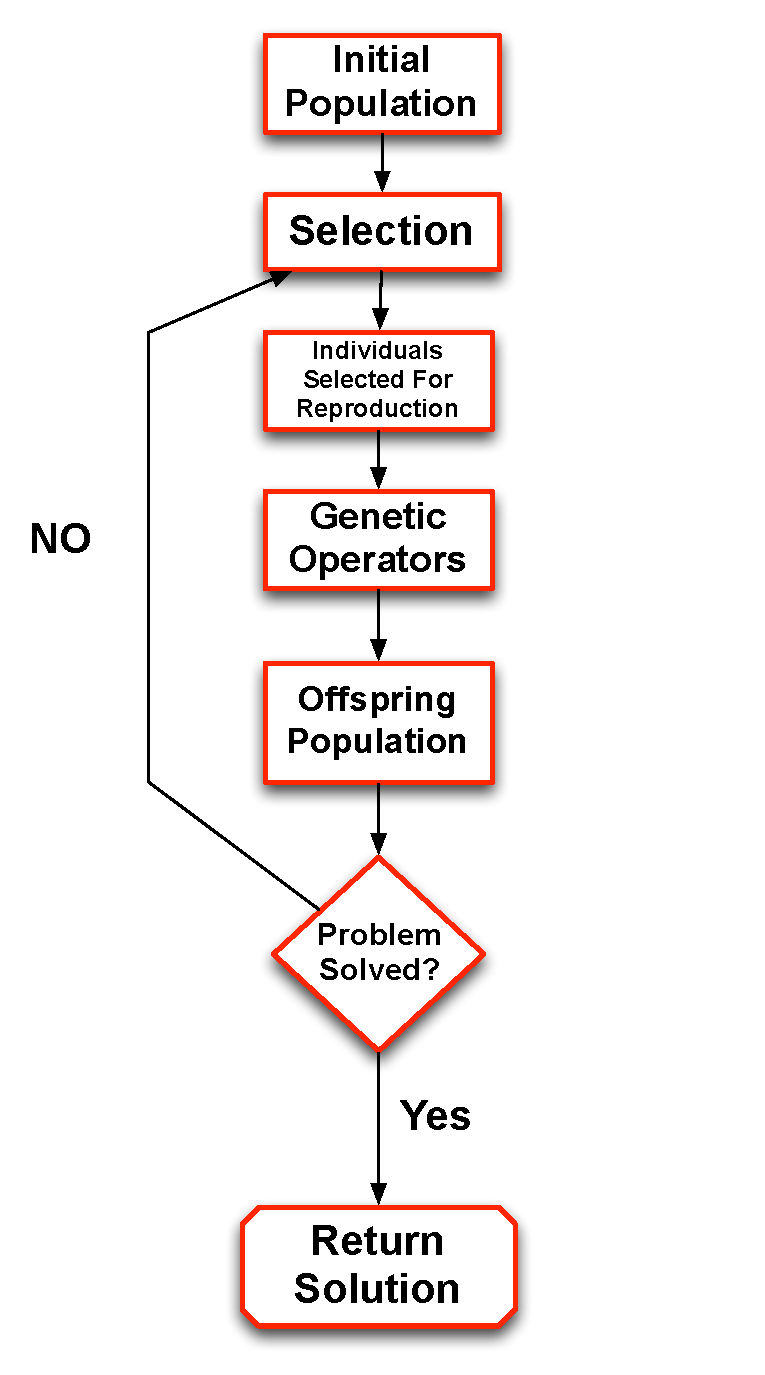
\includegraphics[height=0.85\textheight]{Illustrations/ECdiagram.pdf}
       \\
   \only{\tiny{The Evolutionary Computation Process}}
\end{column}
\end{columns}

\end{frame}
\subsection[Genetic Programming]{Genetic Programming}
\begin{frame}
	\frametitle{Genetic Programming}
\begin{columns}[T]
\begin{column}{0.5\textwidth}
\begin{itemize}	
	\item Genetic programming (GP) uses the EC process to evolve \textbf{programs}
	\item This done by using an Evolutionary Algorithm (EA)
	
	
\end{itemize}
\end{column}
\begin{column}{0.5\textwidth}
   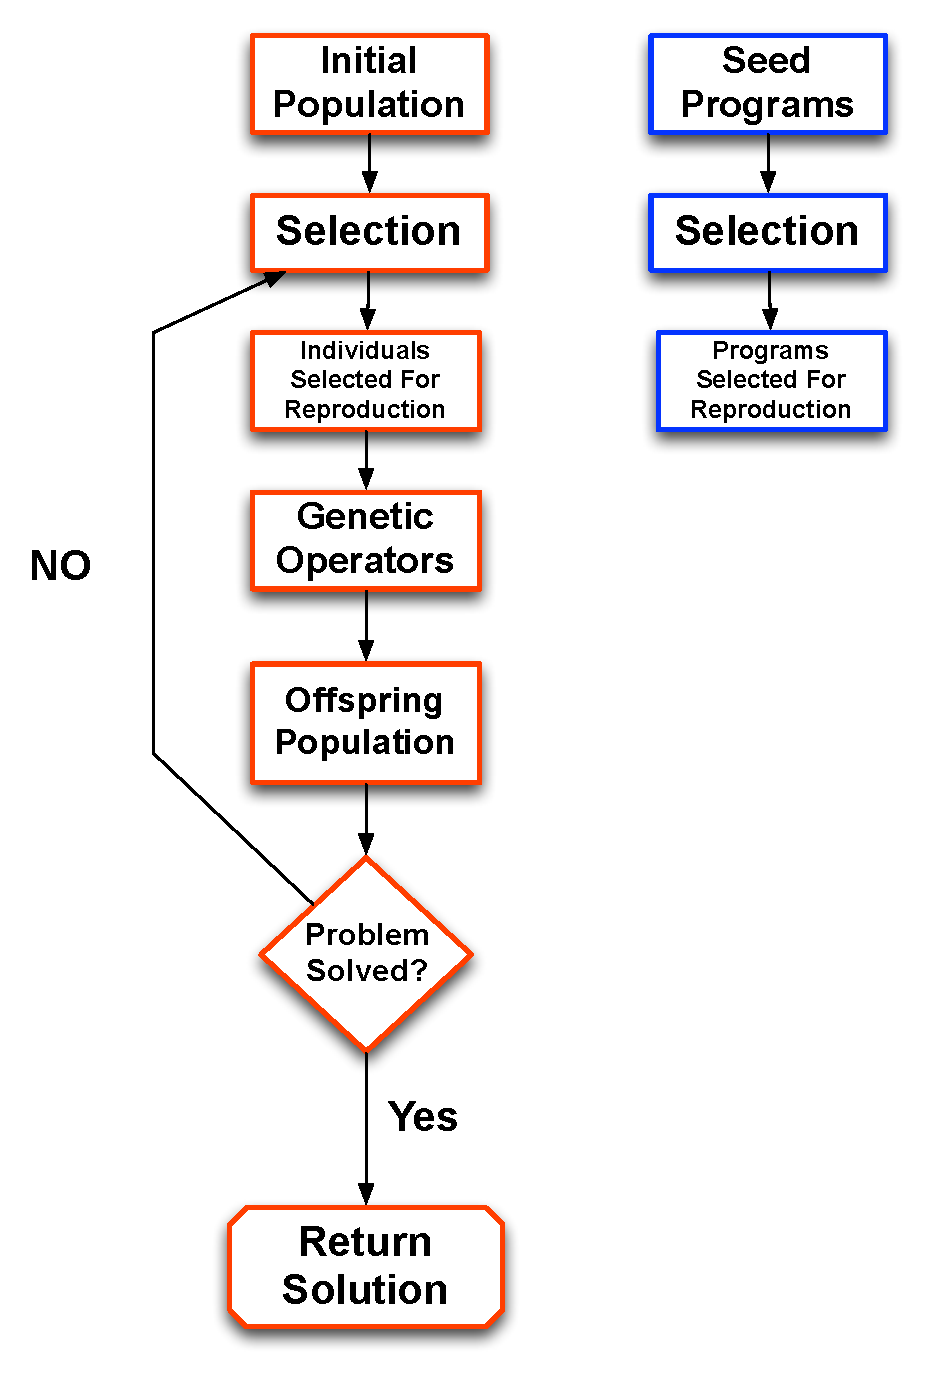
\includegraphics[height=0.85\textheight]{Illustrations/GP2.pdf}

\end{column}
\end{columns}
\end{frame}



\begin{frame}
	\frametitle{Genetic Programming}

\begin{columns}[C]
\begin{column}{0.5\textwidth}


Two genetic operators used in GP are \textit{crossover} and \textit{mutation}


\end{column}
\begin{column}{0.5\textwidth}
   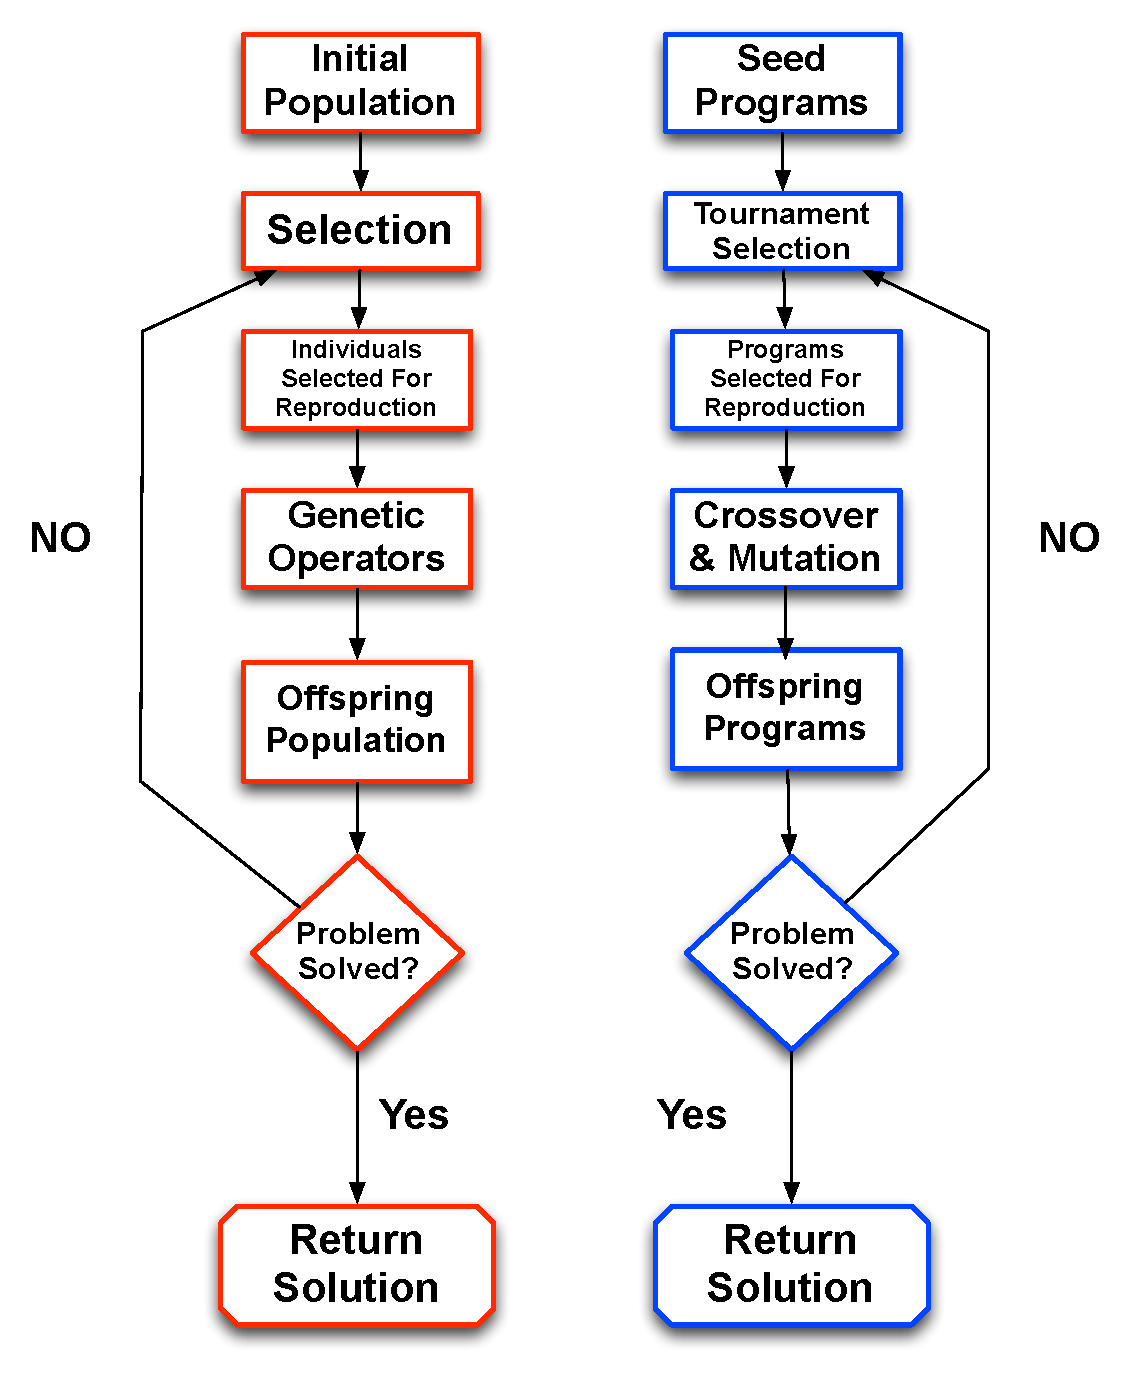
\includegraphics[height=0.85\textheight]{Illustrations/GP3.pdf}

\end{column}
\end{columns}

\end{frame}

\begin{frame}
	\frametitle{Crossover}

   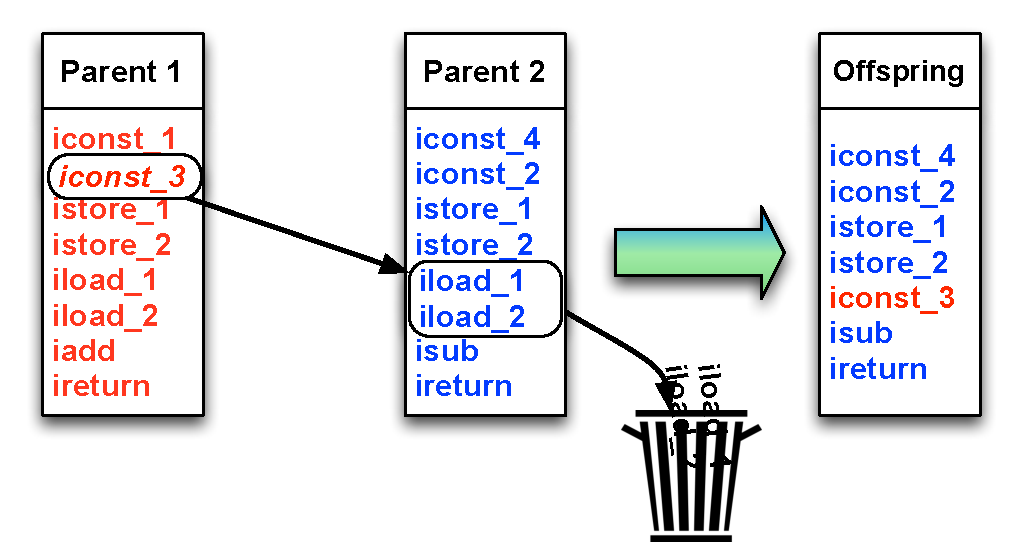
\includegraphics[width=1\textwidth]{Illustrations/crossover.pdf}
       \\
   \only{\tiny{Crossover with Java Bytecode}}

\end{frame}

\begin{frame}
	\frametitle{Mutation}

   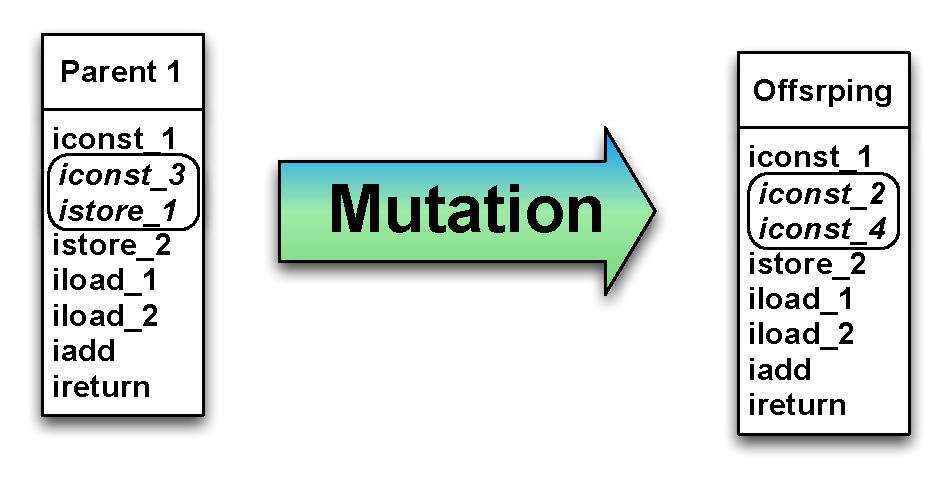
\includegraphics[width=1\textwidth]{Illustrations/mutation.pdf}
       \\
   \only{\tiny{Crossover with Java Bytecode}}

\end{frame}


\section[Why]{Why Byetocde and Assembly?}

\subsection{Difficulties in Source Code}
\begin{frame}
	\frametitle{Source Code Semantic Constraints}
	\begin{itemize}
		\item It is difficult to apply evolution to an entire program in source code
			\\
		\begin{itemize}
			\item Source code is made to simplify reading and writing programs
			\item Source code does not represent the semantic constraints of the program.
		\end{itemize}
	\end{itemize}	
\end{frame}

\begin{frame}
	\frametitle{Syntax vs Semantics}
\begin{itemize}
\item Syntax represents structure
\item Semantics represent meaning
	\\
\begin{description}

\item[Semantically Wrong:] The sun rises in the West.  
\item[Semantically Correct:] The sun rises in the East.
\end{description}
\end{itemize}

\end{frame}


\begin{frame}[fragile]
	\frametitle{Syntax vs Semantics}
	Both (a) and (b) are valid syntactically. However, (b) is invalid semantically.
	
	
   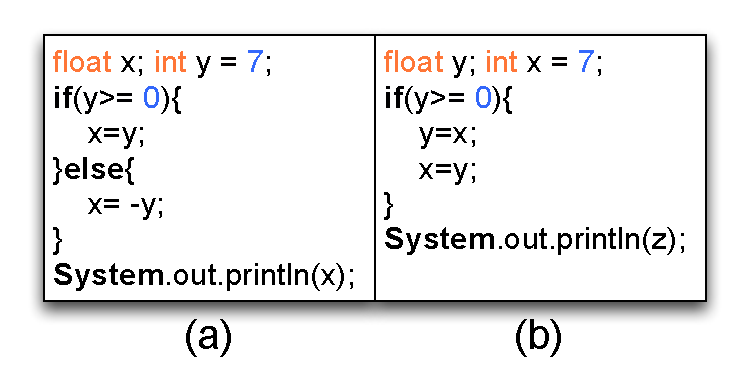
\includegraphics[width=1\textwidth]{Illustrations/semantics.pdf}


\end{frame}




\begin{frame}
	\frametitle{Instruction-Level Code Constraints}
	\begin{itemize}
		\item Consists of a smaller alphabets
		\item Simpler syntactically
		\item Fewer semantic constraints to violate
	\end{itemize}		

\end{frame}




\section[Bytecode and Assembly]{Java Bytecode and the JVM}

\begin{frame}
	\frametitle{Java Virtual Machine}
\begin{columns}
\begin{column}{0.5\textwidth}
\begin{itemize}	
\item A frame stores data and partial results as well as return values for methods
\item Each method call has a frame

\end{itemize}
\end{column}
\begin{column}{0.5\textwidth}
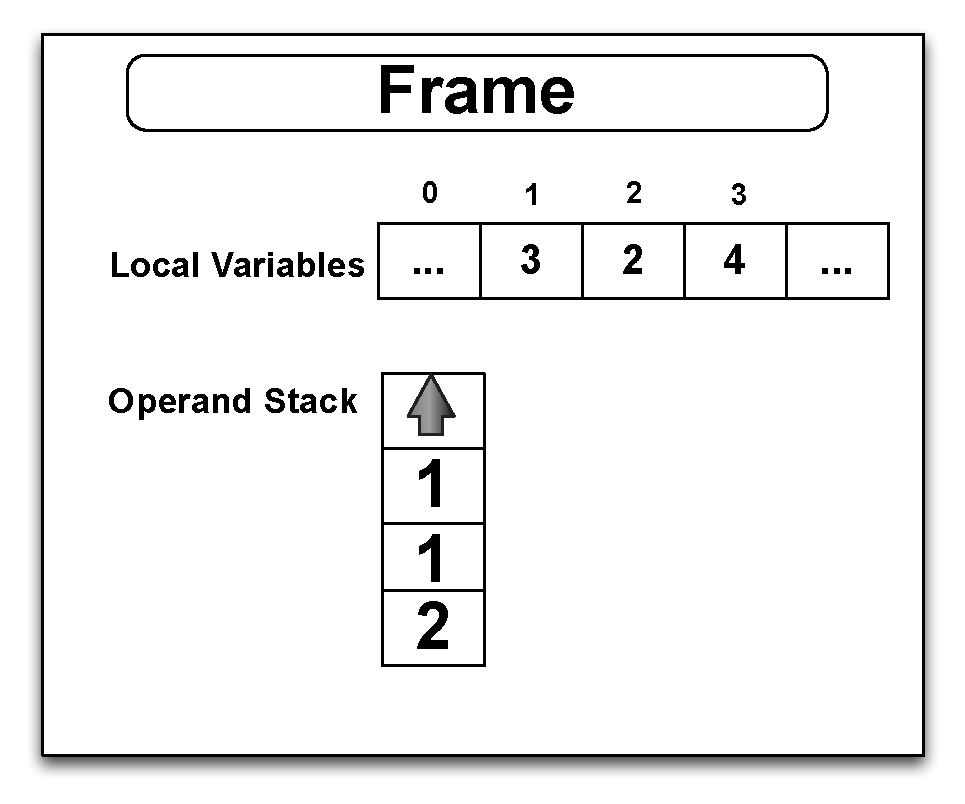
\includegraphics[width=1\textwidth]{Illustrations/frame.pdf}
\end{column}
\end{columns}



\end{frame}



\begin{frame}
\frametitle{Java Bytcode and Frames}
\begin{columns}
\begin{column}{0.5\textwidth}
\begin{itemize}	
\item Opcodes
\item The prefix indicates type
\end{itemize}
\end{column}

\begin{column}{0.5\textwidth}
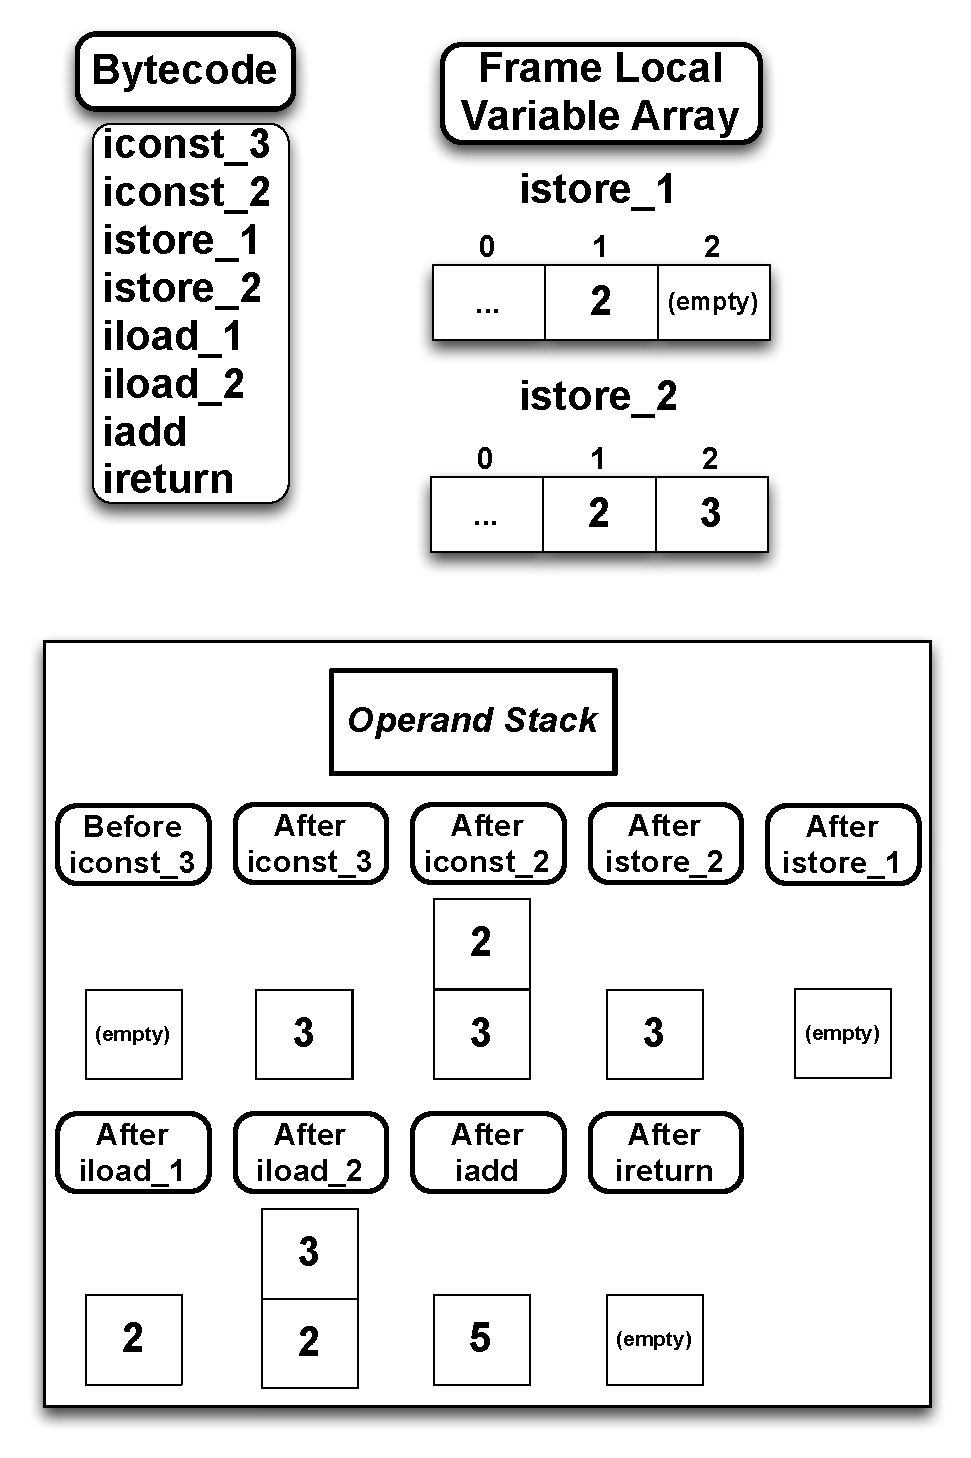
\includegraphics[height=.8\textheight]{Illustrations/stackBytecode.pdf}
\end{column}
\end{columns}
\end{frame}


\section[FINCH]{FINCH:Evolving Java Bytecode}

\subsection[How it works]{How it Works}
\begin{frame}
	\frametitle{What is FINCH?}
	\begin{itemize}
		\item FINCH is an EA developed by Orlov and Sipper	
		\item It evolves Java bytecode
		\item It deals with semantic constraints
	\end{itemize}
\end{frame}

\begin{frame}
  \frametitle{Dealing With Semantic Constraints}
The semantic constraints that are checked for are

	\begin{itemize}
	\item Stack and Frame Depth
	\item Variable Types
	\item Control Flow
	\end{itemize}

\end{frame}

\begin{frame}
\frametitle{Dealing With Semantic Constraints}
\begin{enumerate}
\item Apply crossover to two parents
\item Check if they comply to semantic constraints
\item If the program passes the constraint test then it proceeds to offspring generation
\item If it fails the constraint check then another attempt is made with the same parents
\end{enumerate}

\end{frame}

\begin{frame}
  \frametitle{Bad Crossover}
  \begin{center}
  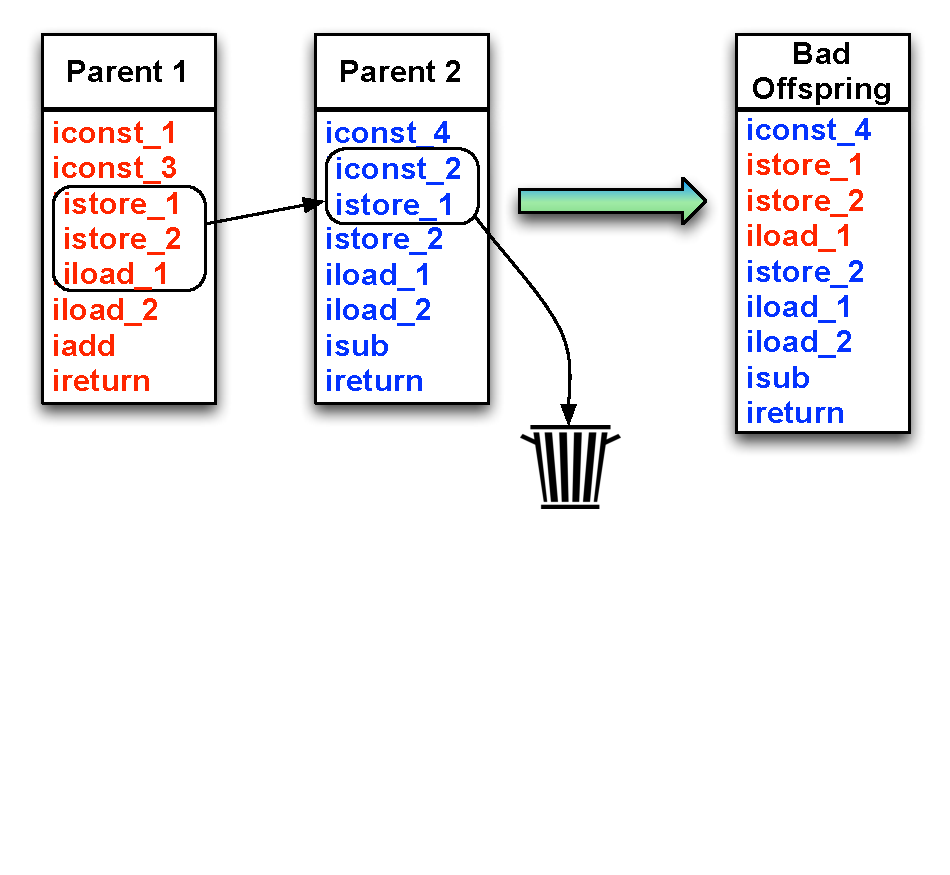
\includegraphics[height=.5\textheight]{Illustrations/badCrossover.pdf}
  \end{center}
  
\end{frame}


\begin{frame}

  \frametitle{Good Crossover}
  \begin{center}
  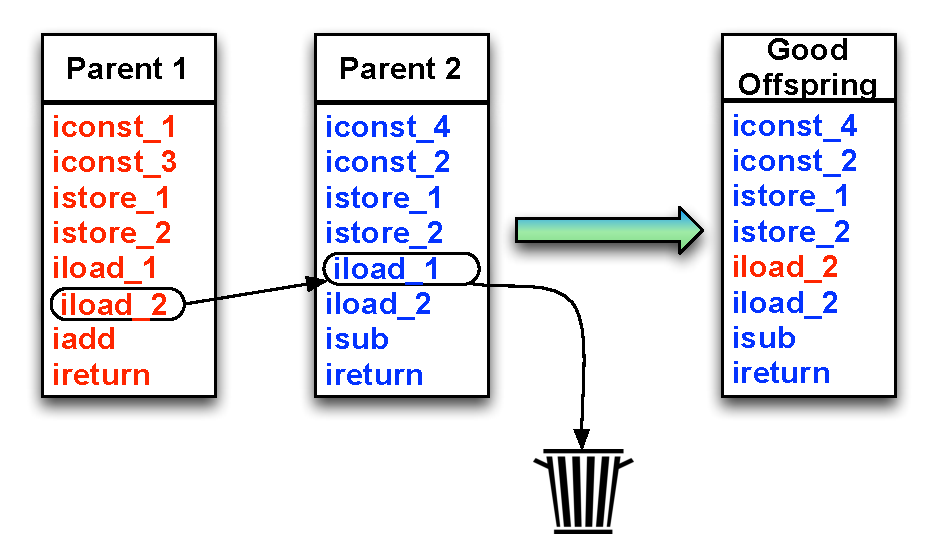
\includegraphics[height=.5\textheight]{Illustrations/goodCrossover.pdf}
  \end{center}
  
\end{frame}



\subsection[The Array Sum Problem]{The Array Sum Problem}

\begin{frame}
\frametitle{Array Sum}
\begin{columns}
\begin{column}{0.5\textwidth}
\begin{itemize}
\item The array sum problem
\\
\begin{itemize}
\item Started with a zero fitness seed program
\item Counted function calls to check for a non-halting state
\end{itemize}

\end{itemize}
\end{column}
\begin{column}{0.5\textwidth}
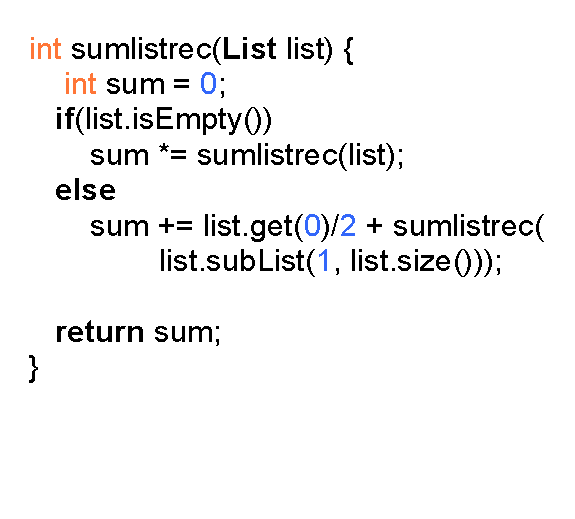
\includegraphics[height=.65\textheight]{Illustrations/seedRec.pdf}
\end{column}
\end{columns}
\end{frame}




\begin{frame}
\frametitle{Array Sum}
\begin{center}
Decompiled Solution
\\
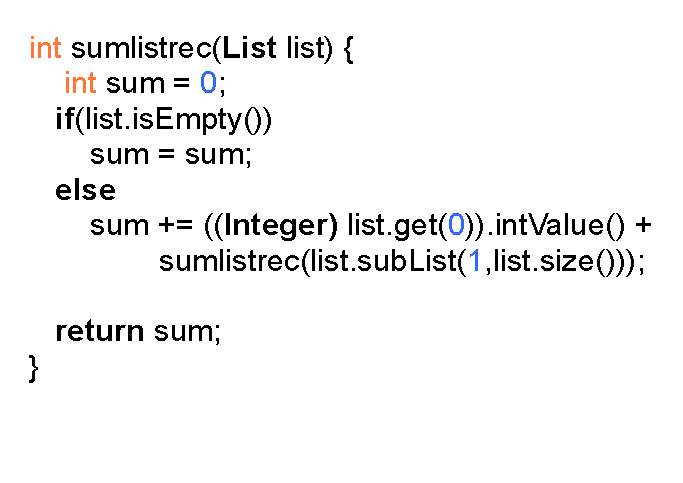
\includegraphics[height=.9\textheight]{Illustrations/solutionRec.pdf}
\end{center}


\end{frame}


\section[Evolving Assembly]{Using Instruction-level Code to Automate Bug Repair}

\subsection{How it Works}
\begin{frame}
  \frametitle{Automating Bug Repair}
  \begin{itemize}
  \item Schulte et al., automated bug repair by evolving Java bytecode and x86 assembly
  \item Fixed bugs in real code
  \item Does not check for semantic constraints 


  \end{itemize}
\end{frame}

\begin{frame}
\frametitle{Tests and Fitness}
\begin{itemize}
	\item Fitness was determined by tests
	\item Test consisted of one \textit{negative} test and multiple \textit{positive} tests
	\item The negative test was used to check if the bug was fixed
\end{itemize}
\end{frame}

\begin{frame}
\begin{itemize}
   \item Programs at times consist of thousands of lines of code  
   \item Uses a weighted path due to size of programs
   \item The weighted path was determined by what tests execute that instruction
\end{itemize}
\end{frame}


\begin{frame}
  \frametitle{Instruction Weight}
  
    \begin{itemize}
  	\item Only executed by failing test: weight = 1.0
  	\item Executed by negative test and one positive: weight = 0.1
  	\item Not executed by negative test case: weight = 0
  \end{itemize}
\end{frame}

\subsection[Results]{Results}

\begin{frame}
\frametitle{What was debugged?}
Schulte et al., were able to debug:
\begin{itemize}
\item Infinite loops
\item Buffer overflows
\item Incorrect type declarations

\end{itemize}


\end{frame}




\section[Conclusions]{Conclusions}

\begin{frame}
\frametitle{Conclusions}


\end{frame}


\begin{frame}
\frametitle{}
{\only<1>{\color{white}}
\cite{FINCH:2011}
\cite{Assembly:2010}
}
\begin{center}
coll0474@morris.umn.edu
\\
\linespace
\linespace
\color{blue}{\fontsize{1cm}{1}\selectfont Questions?}
\end{center}

\end{frame}




\section*{References}

\begin{frame} 
	\frametitle{References} 
	\bibliographystyle{abbrv}
	\bibliography{EricBibliography}
\end{frame} 

\end{document}




